\documentclass{article}

\usepackage[margin=1in, left=1.5in, includefoot]{geometry} 

%graphic stuff
\usepackage{graphicx} % allows images
\usepackage{float} %helps with posisioning

%header and footer stuff
\usepackage{fancyhdr}
\pagestyle{fancy}
\fancyhead{}
\fancyfoot{}
\fancyhead[L]{Software Engineering Group Projects – User Interface Specification Standards / 1.0 (Release)}
\fancyfoot[L]{Aberystwyth University / Computer Science}
\fancyfoot[R]{page: \thepage}
\renewcommand{\headrulewidth}{0pt}
\renewcommand{\footrulewidth}{0pt}

%begins document
\begin{document}

	% begin title screen
	\begin{titlepage}
		\begin{center}
		\line(1,0){340}\\ 
		[0.25in]
		\large{\bfseries Software Engineering Group Project} \\
		\large {\bfseries User Interface Specification Standards}\\
		[2.5mm]
		 \line(1,0){250}\\
		 [0.25in]
		 \textsf {Author: Jor51 and adl12, \\
		 Config Ref: SE.QA.04  \\
		 Date: 22nd December 2016  \\
		 Version: 1.0  \\
		 Status: Release} \\
		 [10.0cm]
		\end{center}
		
		\begin{flushright}
		\textsc {\small Department of Computer Science  \\
		Aberystwyth University  \\
		Aberystwyth  \\
		Ceredigion  \\
		SY23 3DB  \\ 
		Copyright © Aberystwyth University 2016}
		\end{flushright}
	\end{titlepage}
	
	% content section
	\tableofcontents
	\thispagestyle{empty}
	\cleardoublepage	
	\setcounter{page}{1}
	
	%main body section
	\section{introduction} \label{sec:intro}
	This is a documentation on the User interface. It will be going through all the possible use cases and what happens at each screen. Some changes to the layout may be changed at a later date.`
	
	\section{Use case document} \label{sec:usercase}
	\subsection{Typical users}
	For the typical users we will need to design the game for all ages making sure the elderly to the young can understand how to play it whilst making it appealing. The buccaneer board game is based for 8 year olds and upwards. We will also need to consider the types of hardware that this game will be running. For example a cheap android tablet to a big gaming computer. We will be designing the game for the age group of 5 – 99 and the hardware of a standard family computer or laptop.
	
	\subsection{Use cases}
	\subsubsection{Use Case 1, The home screen}
	%image homescreen
		\begin{figure}[H]
		\centering
		\includegraphics[width=15cm,height=13cm,keepaspectratio]{mainmenu2}
		\label{fig:mainmenu}
		\end{figure}
	%content on home screen
	The home screen will allow the user to input 4 player names and have 4 buttons they can click (start, instructions, about and quit).\\

Inputting names and the start button\\
There will be 4 different colour boxes to input the user names, the colour representing the ship colour. If a user doesn’t enter their name it will go to a default name as player 1 for an example. Once the user clicks start it will take the inputted names and begin the game going to the main board screen.\\

Instructions\\
This will bring up another menu with small boxes of each possible event the game will use. For example the chance card or when getting into battle.\\

About\\
The about page will have 3 sections;
The title: the title of the game(buccaneer)
The creators: our group names
Version: to keep up with the updates so we can refer to notes and see what has changed in each version. This will just display a number for example 3.2.\\

Quit\\
This button will exit the game and take the user back to the home screen. Before the application closes itself it will bring up a small menu to make sure the user does want to quit.\\

	\subsubsection{Use Case 2, The main board}
	
		%image Mainboard
		\begin{figure}[H]
		\centering
		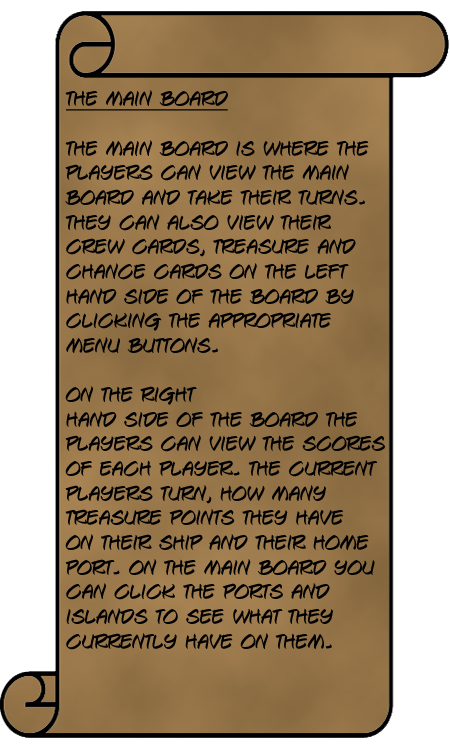
\includegraphics[width=15cm,height=13cm,keepaspectratio]{mainboard}
		\label{fig:mainboard}
		\end{figure}	
	The main board will be where the users can see the board and choose what they do on their turn. This will display 3 clickable options that will bring up menus(cards (crew), chance and treasures). These clickable options will be discussed in more detail further into this document. This means there will be little explanation in this section. 2 options that will allow the user to change their boats position in the highlighted square (move and direction button). There will also be an end turn button.\\
	
	Cards / chance / treasure\\
For the cards section the user can display all the users crew cards which will allow the user to know his or her battle strength and move speed. If the user clicks on chance The game will open a menu up showing the user all there chance cards from their inventory. For treasure another menu will pop up displaying the treasure they are carrying on their ship. \\

Moving and Changing directions\\
The user will be able to move their ship with one of these options. Firstly the user will be able to move. This will highlight all squares in the direction the ship is facing that the ship can move. Once the user clicks a highlighted square the ship will move to that square. After moving the ship can change direction. This will highlight the squares around the ship allowing the user to click to change direction. If a user clicks a non highlighted square an error message will pop up prompting the user to click a highlighted square. \\

End turn\\
Once the user has ran out of turns the user can click the end turn button allowing his turn to end and the next users turn to begin.\\

	\subsubsection{Use Case 3, The crew card menu}
	
		%image crewcard
		\begin{figure}[H]
		\centering
		\includegraphics[width=15cm,height=13cm,keepaspectratio]{crewcard}
		\label{fig:crewcard}
		\end{figure}
		
The crew card menu will allow the user to see how many of each colour card they have. The application will also calculate the movement and the attack power of the users ship. if the user gets more than 8 cards the user will be able to use the scroll bar to see the rest of his cards. once the user is satisfied they can use the x in the top right corner to close the menu and get back to the main board. \\

	\subsubsection{Use Case 4, The chance card menu}
	
		%image chancecard
		\begin{figure}[H]
		\centering
		\includegraphics[width=15cm,height=13cm,keepaspectratio]{chancecard}
		\label{fig:chancecard}
		\end{figure}
	
	The chance card menu will allow the user to see all Their chance cards they have stored in their inventory. If a player would like to activate a card the user would click the card they would like to use then click activate. This will take them back to the board screen with the chance card activated. If a user has more than 8 chance cards stored the user will be able to scroll down the menu. if the user would like to exit they would click the x in the top corner and that will take them back to the main board to continue their turn.
	
	\subsubsection{Use Case 5, The treasure card menu}
	
		%image treasurecard
		\begin{figure}[H]
		\centering
		\includegraphics[width=15cm,height=13cm,keepaspectratio]{treasurecard}
		\label{fig:Treasurecard}
		\end{figure}	
		
		The treasure card menu will display the treasure you have in your ship. This will display 2 images giving you the value of points on per image. The application will also add them up if possible and display them as the total. Once the user is ready they can click the x in the top corner to close the application. if the user only has 1 or even no treasures the unnecessary squares will become transparent so only the background displays.
	
	\subsubsection{Use Case 6, The battle screen menu}
	
		%image Battlescreen
		\begin{figure}[H]
		\centering
		\includegraphics[width=15cm,height=13cm,keepaspectratio]{battle}
		\label{fig:battle}
		\end{figure}
	
When a player moves to a occupied square due to another player they can battle. Once the ship is on the occupied square the battle window will pop out and display the following information. The 2 users who are currently in the battle phase display name. a display picture of there coloured boat. The screen will display the attack power and the winners users name in the winner box, and a collect rewards box allowing the user to collect their reward. 

	\subsubsection{Use Case 7, The battle reward screens}
	
	When you have won a battle there are 2 possible rewards. These are the treasure reward and the crew reward. If a user beats the ship in battle they get to take a treasure. If the ship that lost contains no treasure the user will be given 2 of the other ships lowest crew automatically. If the ship has treasure but the victorious ship has full treasure the losers treasure goes to treasure island where a pop up will pop out telling the users the treasure has been returned to treasure island.
	
		%image treasurereward
		\begin{figure}[H]
		\centering
		\includegraphics[width=15cm,height=13cm,keepaspectratio]{rewardtreasure}
		\label{fig:treasureprize}
		\end{figure}

For the treasure reward if the victorious player already has a treasure then one of the boxes would become transparent so only one displays. Once the box has been clicked the user will select the treasure they are after from the opponent. Once the user is happy with the selection the user can click the ok button to gain the selected treasure and to go back to the main board.

	%image crewrewards
		\begin{figure}[H]
		\centering
		\includegraphics[width=15cm,height=13cm,keepaspectratio]{rewardcrew}
		\label{fig:crewreward}
		\end{figure}
		
		For the crew reward as it is the lowest crew the application will display the 2 lowest crew members from the losers inventory  and once you have clicked ok the crew will be transferred to your collection.
		
	
	\subsubsection{Use Case 8, The Trading screen}
	
		%image trading
		\begin{figure}[H]
		\centering
		\includegraphics[width=15cm,height=13cm,keepaspectratio]{trading}
		\label{fig:trading}
		\end{figure}	
		
When a player moves to a trade port they can trade. Once the ship is on the trade port square a window will pop out and display the following information. The window will be split in two one side displaying the users treasure and crew cards and the other displaying the treasure and crew cards the port has. Each side will have a scroll bar to
be able to scroll up and down and view all of the cards if there is too many to fit on the screen. There will be 2 values showing the value of the treasure and crew cards selected from each side above the two lists this to help the user see what values they've picked to swap and to help them match the numbers and make a trade. When a picture of the crew
card or treasure is clicked it will highlighted and added to the proposed trade the value of that item will be added to the value at the top. There will be two buttons in the middle of these 2 sides a Accept button and a Decline button. When the two values 
match the accept button will be able to be clicked one this button is clicked the window will close and the trade will have happened. If the decline button is clicked the trade window will close and no trade will happen.

\subsubsection{Use Case 9, Treasure Gained screen}
	
		%image treasuregained
		\begin{figure}[H]
		\centering
		\includegraphics[width=15cm,height=13cm,keepaspectratio]{treasuregain}
		\label{fig:treasuregain}
		\end{figure}

When the player is allowed to choose treasure to get a window will pop out to allow them to do this. This window will have a picture of each treasure 
available. The pictures can be clicked to select that treasure to take and it will highlight the treasure that has been picked. There will be scroll bar
to allow for if there is too much treasure to fit onto one page. There will be a value at the top of the page displaying the total value of the treasure 
picked so far. The number of treasure that can be picked is the amount of space the have left in their ship. When the treasure under the max value is 
picked an accept button at the bottom right of the window will be allowed to be clicked and this will then close the window and award the treasure to the
player. For cases when taking crew cards instead is an option there will be an additional button above the accept to take the set number of crew cards. 
This button will close the window and assign the crew cards to the player.	

\subsubsection{Use Case 10, Victory Screen}

%image victory
		\begin{figure}[H]
		\centering
		\includegraphics[width=15cm,height=13cm,keepaspectratio]{victory}
		\label{fig:victory}
		\end{figure}
		
When a player wins (gets 20 or more points) the main board window will change to a victory window. On this window will be "winner", the name of the player, a 
picture of the players ship and 2 buttons one for play again and one for close. The background of this window will have fireworks. If the play again button
is clicked then the game resets and returns to the home screen (see use case "enter number here"). If the close button is clicked then the program stops and closes.


\subsubsection{Use Case 11, Picking a player}

When the game requires a player to pick another player for an action to happen against a window will pop out. It will have a picture of other players boat and their
name underneath the boat. When a player clicks a player they will be highlighted and an accept button will be allowed to be clicked in the bottom left. When the accept
button is clicked the window closes and the action happens to that player. 



\subsubsection{Use Case 12, Long John Silver}

When a player with the chance card long john silver sails into a trade port a window will pop out that looks identical to use case "enter number of gaining treasure here"
except the user will not be presented with treasure but rather crew cards and the value at the top will measure the value of the crew cards they have picked. When a player
enters a port where Long John Silver and have treasure to be able to trade a window will pop out asking if they want to trade a treasure for the chance card. A button for
no and yes will on this window if no is clicked then the player keeps there treasure and the chance card stays in the port if yes is clicked then the trade for the chance
card happens. The window closes after each of these options are clicked. 



\subsubsection{Use Case 13, Special Trade Cards}

When a player has a chance card such as number 23 or 24 in the requirements specification and enters a trade port a window the same as use case "enter number for long john silver here"
will pop out. If yes is selected this window closes and a window the same as use case "enter number for gaining treasure up to a value here" this will display the 
crew cards and the treasure that the port has. The player will then be able to click treasure or crew (but not both) and the value at the top will increase 
by the value of the crew or treasure that was chosen. When the player has selected treasure (that they can hold) or crew cards under the set value the accept button
can be clicked and when it is the window will close and the treasure or crew are assigned to the player.


	\subsection{Error conditions}
	error conditions are small error boxes that pop up giving the user a brief description of what has gone wrong when a user uses the application incorrectly.
	\subsubsection{Error conditions for the main page}
	
\begin{table}[H]
\centering
\caption{main page}
\label{error main page}
\resizebox{\textwidth}{!}{%
\begin{tabular}{ll}
Player name too long or short & Please type a name that is between 3 - 10 characters long. \\
No player name was entered in a field  & Please make sure all 4 players name boxes are filled out.  \\
Character for user name not applicable &  Please make sure you use English letters only and no special characters \\
 
\end{tabular}%
}
\end{table}

\subsubsection{Chance cards}
	
\begin{table}[H]
\centering
\caption{Error conditions on main page}
\label{error main page}
\resizebox{\textwidth}{!}{%
\begin{tabular}{ll}
If there is a requirement and cant use the card & Please read the card and activate when applicable
 
\end{tabular}%
}
\end{table}

\end{document}